\documentclass[border=4pt]{standalone}
% Preámbulo común de las figuras. Cada figura es un documento standalone
% que se compila a SVG con scripts/build_figures.sh
\usepackage[utf8]{inputenc}
\usepackage{amsmath}
\usepackage{tikz}
\usepackage[american, siunitx]{circuitikz}
\usetikzlibrary{arrows.meta,calc,decorations.pathmorphing,patterns}
\tikzset{
  >={Stealth[length=2.2mm]},
  eje/.style={->, thin},
  hilo/.style={thick},
}
% Paleta común: tonos medios legibles sobre fondo claro
\definecolor{azul}{RGB}{31,94,168}
\definecolor{rojo}{RGB}{192,57,43}
\definecolor{verde}{RGB}{39,128,73}
\definecolor{naranja}{RGB}{211,120,30}
\definecolor{morado}{RGB}{125,60,152}

\begin{document}
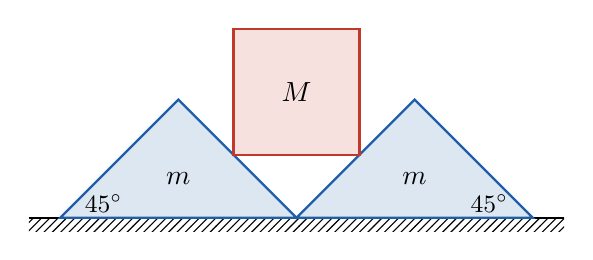
\begin{tikzpicture}[scale=1.0]
  \fill[pattern=north east lines] (-0.4,-0.18) rectangle (6.4,0);
  \draw[thick] (-0.4,0) -- (6.4,0);
  % cuñas: triángulos rectángulos isósceles con el ángulo recto arriba
  \filldraw[draw=azul, fill=azul!15, thick] (0,0) -- (3,0) -- (1.5,1.5) -- cycle;
  \filldraw[draw=azul, fill=azul!15, thick] (3,0) -- (6,0) -- (4.5,1.5) -- cycle;
  \node at (1.5,0.5) {$m$};
  \node at (4.5,0.5) {$m$};
  % cubo sin girar: sus esquinas inferiores se apoyan en las caras interiores
  % (y = 3 - x, y = x - 3) y queda separado del piso
  \filldraw[draw=rojo, fill=rojo!15, thick] (2.2,0.8) rectangle (3.8,2.4);
  \node at (3,1.6) {$M$};
  \node[font=\small] at (0.55,0.18) {$45^\circ$};
  \node[font=\small] at (5.45,0.18) {$45^\circ$};
\end{tikzpicture}
\end{document}
